
\chapter{Congruence Path Refinement}
\label{chap:pr}

\section{Theory}

Before we present the path refinement method, note that it takes a special case as it is only defined for state pairs within one DPA, not between different automata.

\begin{defn}
	Let $\mathcal{A} = (Q, \Sigma, \delta, c)$ be a DPA and let $R \subseteq Q \times Q$ be a congruence relation on the state space. Let $\lambda \subseteq Q$ be an equivalence class of $R$. We define $L_{\lambda \hookleftarrow}$ as the set of non-empty words $w$ such that for all $q \in \lambda$ and all $u \sqsubseteq w$, $(\delta(q, u), q) \in R$ iff $u \in \{\varepsilon, w\}$. In other words, the set contains all minimal words by which the automaton moves from $\lambda$ to $\lambda$ again.
	
	Let $f_\text{PR} : 2^{\lambda \times \lambda} \rightarrow 2^{\lambda \times \lambda}$ be a function such that $(p, q) \in f_\text{PR}(X)$  iff for all $w \in L_{\lambda \hookleftarrow}$, $(\delta^*(p, w), \delta^*(q, w)) \in X$.
	Then let $X_0 \subseteq \lambda \times \lambda$ such that $(p, q) \in X_0$ iff for all $w \in L_{\lambda \hookleftarrow}$, $\min \{ c(\delta^*(p, u)) \mid u \sqsubseteq w \} = \min \{ c(\delta^*(q, u)) \mid u \sqsubseteq w \}$, i.e. the minimal priority when moving from $p$ or $q$ to $\lambda$ again is the same.
	
	Using both, we set $X_{i+1} = f_\text{PR}(X_i)$. $f_\text{PR}$ is monotone w.r.t. $\subseteq$, so there is an $X_n = X_{n+1}$ by Tarski's fixed point theorem (\cite{Tarski1955}). We define the \emph{path refinement of $\lambda$}, called $\equiv_\text{PR}^\lambda$, as
	\begin{itemize}
		\item For $p \in Q \setminus \lambda$, $p \equiv_\text{PR}^\lambda q$ iff $p = q$.
		\item For $p, q \in \lambda$, $p \equiv_\text{PR}^\lambda q$ iff $(p, q) \in X_n$.
	\end{itemize}
\end{defn}

$\lambda$ being an equivalence class of $R$, a congruence relation, is required for the definition of $L_{\lambda \hookleftarrow}$ to be consistent.

\vspace{5pt}

\begin{lem}
	$\equiv_\text{PR}^\lambda$ is an equivalence relation.
\end{lem}

\begin{proof}
	The disjoint union of two equivalence relations is an equivalence relation, so we only focus on $\lambda$ here; it is obvious that $\equiv_\text{PR}^\lambda$ is an equivalence relation on $Q \setminus \lambda$.
	
	We can actually observe that every $X_i$ is an equivalence relation. For $X_0$ this is true as that relation is solely defined by equivalence of values. Then by induction it easily follows if $X$ is an equivalence relation that $f_\text{PR}(X)$ is one as well.
\end{proof}

\begin{defn}
	Let $\mathcal{A}$ be a DPA. We define the \emph{path refinement merger} as $$\mu_\text{PR}^\lambda : \{ \kappa \in \mathfrak{C}(\equiv_\text{PR}^\lambda, \mathcal{A}) \mid \kappa \subseteq \lambda \} \rightarrow 2^Q, \kappa \mapsto \{ q \in \kappa \mid c(q) = \min c(\kappa) \}.$$
\end{defn}

\vspace{10pt}

\begin{theorem}
	Let $\mathcal{A}'$ be a representative merge of a DPA $\mathcal{A}$ w.r.t $\mu_\text{PR}^\lambda$. If all states in $\lambda$ are pairwise language equivalent, then $(\mathcal{A}, q) \equiv_L (\mathcal{A}', q)$ for all $q \in Q'$.
	\label{thm:pr:preserves_language}
\end{theorem}

\begin{proof} 
	Let $\alpha \in \Sigma^\omega$ be a word with runs $\rho \in Q^\omega$ and $\rho' \in (Q')^\omega$ of $\mathcal{A}$ and $\mathcal{A}'$ respectively, starting in the same state. Let $k_0, \dots \in \mathbb{N}$ be exactly those positions (in order) at which $\rho$ reaches $\lambda$, and analogously $k'_0, \dots$ for $\rho'$. 

	\vspace{5pt}
	\textbf{Claim 1}: For every $i$, $k_i = k'_i$ and $\rho(k_i) \equiv_\text{PR}^\lambda \rho'(k_i)$. \\
	For all $j < k_0$, we know that $\rho(j) = \rho'(j)$, as no redirected edge is taken. Thus, $\rho'(k_0) = r_{[\rho(k_0)]_{\equiv_\text{PR}^\lambda}} \equiv_\text{PR}^\lambda = \rho(k_0)$.
	
	Now assume that the claim holds for all $i \leq n$. By definition, $w = \alpha[k_n, k_{n+1}] \in L_{\lambda \hookleftarrow}$ and therefore $\rho(k_{n+1}) = \delta^*(\rho(k_n), w) \equiv_\text{PR}^\lambda \delta^*(\rho'(k_n), w) = \rho'(k_{n+1})$.
	
	\vspace{5pt}
	\textbf{Claim 2}: If $\lambda$ only occurs finitely often in $\rho$ and $\rho'$, then $\rho$ is accepting iff $\rho'$ is accepting. 
	
	Let $k_n \in \mathbb{N}$ be the last position at which $\rho(k_n)$ and $\rho'(k_n)$ are in $\lambda$. From this point on, $\rho'[k_n, \omega]$ is also a valid run of $\mathcal{A}$ on $\alpha[k_n, \omega]$. As states in $\lambda$ are language equivalent, reading $\alpha[k_n, \omega]$ from either state $\rho(k_n)$ or $\rho'(k_n)$ in $\mathcal{A}$ leads to the same acceptance status. This also means that $\rho'(k_n)$ has the same acceptance status as $\rho(k_n)$.
	
	\vspace{5pt}
	\textbf{Claim 3}: If $\lambda$ occurs infinitely often in $\rho$ and $\rho'$, then $\rho$ is accepting iff $\rho'$ is accepting. 
	
	We abbreviate $\text{Occ}(c(\rho[x, y])) = O[x, y]$ and $\text{Occ}(c(\rho'[x, y])) = O'[x, y]$. $c$ and $c'$ map all states to the same values by definition of the merge, so $c'(\rho'(i))$ and $c(\rho'(i))$ are the same.
	
	First, observe that for all $i$, $\min O[k_i, k_{i+1} + 1] \geq \min O'[k_i, k_{i+1} + 1]$: By definition of $\equiv_\text{PR}^\lambda$, all states within an equivalence class visit the same minimal priority on their way from $\lambda$ back to $\lambda$ (in $\mathcal{A}$). In particular, $\rho(k_i)$ and $\rho'(k_i)$ do. That means $\min O[k_i, k_{i+1} + 1] = \min O'[k_i, k_{i+1}] \cup c(p_{i+1})$, where $p_{i+1} = \delta(\rho'(k_{i+1}), \alpha(k_{i+1}))$. By choice of the candidates of the merge, $c(p_{i+1}) \geq c(\rho'(k_{i+1}))$, so $\min O'[k_i, k_{i+1}] \cup c(p_{i+1}) \geq \min O'[k_i, k_{i+1} + 1]$. We can extend this to $\min \text{Inf}(c(\rho)) \geq \min \text{Inf}(c(\rho'))$.
	
	Now assume that there is a priority $l$ in $c(\rho')$ that occurs infinitely often but only finitely often in $c(\rho)$. Let this priority be minimal and let $k_m$ be a position with $c(\rho'(k_m)) = l$ but $l$ never occurs in $c(\rho)$ at or after position $k_m$.
	
	We still have $\rho(k_m) \equiv_\text{PR}^\lambda \rho'(k_m)$, so $\min O[k_m, k_{m+1} + 1]$ and $\min O'[k_m, k_{m+1}] \cup \{c(p_{m+1})\}$ must be the same. Obviously, $l$ is an element of $O'[k_m, k_{m+1}]$, so a priority at most as high as $l$ is visited in $\rho[k_m, k_{m+1} + 1]$. This happens every time $l$ is seen in $c(\rho')$, so $l > \min \text{Inf}(c(\rho'))$. As $l$ was the smallest priority that differs between the two infinity sets, their minimum must be the same.
\end{proof}



\section{Computation}
The definition of path refinement that we introduced is useful for the proofs of correctness. It however does not provide one with a way to actually compute the relation. That is why we now provide an alternative definition that yields the same results but is more algorithmic in nature.

\begin{defn}
	Let $\mathcal{A} = (Q, \Sigma, \delta, c)$ be a DPA and let $R \subseteq Q \times Q$ be a congruence relation. For each equivalence class $\lambda$ of $R$, we define the \emph{path refinement automaton} \linebreak $\mathcal{G}_\text{PR}^\lambda(p, q) = (Q_\text{PR}, \Sigma, \delta^\lambda_\text{PR}, F_\text{PR})$, which is a DFA.
	
	\begin{itemize}
		\item $Q_\text{PR} = (Q \times Q \times c(Q) \times \{<, >, =\}) \cup \{ \perp \}$
		\item $\delta^\lambda_\text{PR}((p, q, k, x), a) = \begin{cases}
			(p', q', \eta_k(c(p'), c(q'), k), \eta_x(c(p'), c(q'), k, x)) & \text{if } p' \notin \lambda \\
			q_0^\text{PR}(p', q') & \text{if } p' \in \lambda \text{ and } \\ 
			& \quad (\eta_x(c(p'), c(q'), k, x) =\, =) \\
			\perp & \text{else}
		\end{cases}$ \\
			where $p' = \delta(p, a)$ and $q' = \delta(q, a)$. \\
			$\eta_k(k_p, k_q, k) = \min_{\leq_\checkmark} \{k_p, k_q, k\}$ \\
			$\eta_x(k_p, k_q, k, x) = \begin{cases}
				< & \text{if } (k_p <_\checkmark k_q \text{ and } k_p <_\checkmark k) \text{ or } (k < k_q \text{ and } (x =\, <)) \\
				> & \text{if } (k_p >_\checkmark k_q \text{ and } k >_\checkmark k_q) \text{ or } (k_p > k \text{ and } (x =\, >)) \\
				= & \text{else}
			\end{cases}$ 
		\item $F_\text{PR} = Q_\text{PR} \setminus \{\perp\}$
	\end{itemize}

	We use the following initial state for $p, q \in \lambda$: $$q_0^\text{PR}(p, q) = (p, q, \eta_k(c(p), c(q), \checkmark), \eta_x(c(p), c(q), \checkmark, =))$$
\end{defn}

\begin{lem}
	Let $p$ and $q$ be two states in $\lambda$ and let $w$ be a word in $L_{\lambda \rightarrow \lambda}$. For every $v \sqsubset w$ and \linebreak
	$\oplus \in \{<, >, =\}$, the fourth component of $(\delta_\text{PR}^\lambda)^*(q_0^\text{PR}(p, q), v)$ is $\oplus$ if and only if \linebreak
	$\min \{ c(\delta^*(p, u)) \mid u \sqsubseteq v \} \oplus \min \{ c(\delta^*(q, u)) \mid u \sqsubseteq v \}$.
	\label{lem:pr:pr_game_nx}
\end{lem}
\vspace{5pt}
	The proof of this Lemma is a very formal analysis of every case in the relations between the different priorities that occur and making sure that the definition of $\eta_x$ covers these correctly. No great insight is gained, which is why we omit the proof at this point.

\begin{theorem}
	Let $p, q \in \lambda$. Then $p \equiv_\text{PR}^\lambda q$ iff $L(\mathcal{G}_\text{PR}^\lambda(p, q), q_0^\text{PR}(p, q)) = \Sigma^*$.
\end{theorem}

\begin{proof}
	\textbf{If } Let $p \not\equiv_\text{PR}^R q$. We use the inductive definition of $R_\kappa \subseteq\, \equiv_\text{PR}^R$ using $f$ and the sets $X_i$ here. Let $m$ be the smallest index at which $(p, q) \notin X_m$. Let $\rho = (p_i, q_i, k_i, x_i)_{0 \leq i \leq |w|}$ be the run of $\mathcal{G}_\text{PR}^\lambda(p, q)$ on $w$. We prove that $\rho(|w|) = \perp$ and therefore $\rho$ is not accepting by induction on $m$.
	
	If $m = 0$, then $(p, q) \notin Y_\lambda$, meaning that there is a word $w$ such that $\min \{ c(\delta^*(p, u)) \mid u \sqsubset w \} \neq \min \{ c(\delta^*(q, u)) \mid u \sqsubset w \}$. Without loss of generality, assume $\min \{ c(\delta^*(p, u)) \mid u \sqsubset w \} < \min \{ c(\delta^*(q, u)) \mid u \sqsubset w \}$. By Lemma \ref{lem:pr:pr_game_nx}, $x_{|w|-1} =\, <$. Furthermore, $\delta(p_{|w|-1}, w_{|w|-1}) \in \lambda$, as $w \in L_{\lambda \rightarrow \lambda}$. Thus, $\rho(|w|) =\, \perp$ and the run is rejecting.
	
	Now consider $m+1 > 1$. Since $(p, q) \in X_m \setminus f(X_m)$, there must be a word $w \in L_{\lambda \rightarrow \lambda}$ such that $(p', q') \notin X_m$, where $p' = \delta^*(p, w)$ and $q' = \delta^*(q, w)$. As $R_\kappa \subseteq X_m$, $(p', q') \notin R_\kappa$ and therefore $p' \not\equiv_\text{PR}^R q'$. By induction, $w \notin L(\mathcal{G}_\text{PR}^\lambda(p', q'), q_0^\text{PR}(p', q'))$; since that run is a suffix of $\rho$, $\rho$ itself is also a rejecting run.
	
	\paragraph{Only If} Let $L(\mathcal{G}_\text{PR}^\lambda(p, q), q_0^\text{PR}(p, q)) \neq \Sigma^*$. Since $\varepsilon$ is always accepted, there is a word $w \in \Sigma^+ \setminus L(\mathcal{G}_\text{PR}^\lambda(p, q), q_0^\text{PR}(p, q))$, meaning that $\delta_\text{PR}^*(q_0^\text{PR}(p, q), w) = \perp$. Split $w$ into sub-words $w = u_1 \cdots u_m$ such that $u_1, \dots, u_m \in L_{\lambda \rightarrow \lambda}$. Note that this partition is unique. We show $p \not\equiv_\text{PR}^R q$ by induction on $m$. Let $\rho = (p_i, q_i, k_i, x_i)_{0 \leq i < |w|}$ be the run of $\mathcal{G}_\text{PR}^\lambda(p, q)$ on $w$ starting in $q_0^\text{PR}(p, q)$.
	
	If $m = 1$, then $w \in L_{\lambda \rightarrow \lambda}$. Since $\rho(|w|) =\, \perp$, it must be true that $x_{|w|-1} \neq\, =$. Without loss of generality, assume $x_{|w|-1} =\, <$. By Lemma \ref{lem:pr:pr_game_nx}, $\min \{ c(\delta^*(p, u)) \mid u \sqsubseteq w \} < \min \{ c(\delta^*(q, u)) \mid u \sqsubseteq w \}$. Therefore, $p \not\equiv_\text{PR}^R q$.
	
	Now consider $m+1 > 1$. Let $p' = \delta^*(p, u_1)$ and $q' = \delta^*(q, u_1)$. By induction on the word $u_2 \cdots u_m$, $p' \not\equiv_\text{PR}^R q'$. Since $u_1 \in L_{\lambda \rightarrow \lambda}$, that also means $p \not\equiv_\text{PR}^R q$.
\end{proof}

\vspace{5pt}
The automaton $\mathcal{G}_\text{PR}^\lambda$ has size $\mathcal{O}(|Q|^2 \cdot |c(Q)|)$. For each class $\lambda$, the problem of universal language has to be solved which is solved by reachability in linear time. Thus, $\equiv_\text{PR}^\lambda$ can be computed in time $\mathcal{O}(|Q|^2 \cdot |c(Q)|)$ but has to be repeated for every different $\lambda$.



\section{Faster Computation}
The computation presented in the previous section was a straight-forward description of $\equiv_\text{PR}^\lambda$ in an algorithmic way. We can reduce the complexity of that computation by taking a more indirect route, as we will see now.

\begin{defn}
	Let $\mathcal{A} = (Q, \Sigma, \delta, c)$ be a DPA. Let $R$ be a congruence relation on $Q$ and let $\lambda \subseteq Q$ be an equivalence class of $R$. We define a deterministic transition structure $\mathcal{A}^\lambda_\text{visit} = (Q^\lambda_\text{visit}, \Sigma, \delta^\lambda_\text{visit})$ as follows:
	
	\begin{itemize}
		\item $Q^\lambda_\text{visit} = ((Q \setminus \lambda) \times c(Q) \times \{\perp\}) \cup (\lambda \times c(Q) \times c(Q))$ \\
		These states \enquote{simulate} $\mathcal{A}$ and use the second component to track the minimal priority that was seen since a last visit to $\lambda$. The states in $\lambda$ itself also have a third component that is used to distinguish their classes, as is explained below.
		\item $\delta^\lambda_\text{visit}((q, k, k'), a) = \begin{cases}
			(q', \min \{k, c(q')\}, \perp) & \text{if } q' \notin \lambda \\
			(q', c(q'), \min \{k, c(q')\}) & \text{if } q' \in \lambda
		\end{cases}$, where $q' = \delta(q, a)$.
	\end{itemize}
\end{defn}

\begin{defn}
	Consider $\mathcal{A}^\lambda_\text{visit}$ of a DPA $\mathcal{A}$ and a congruence relation $R$. We define an equivalence relation $V \subseteq Q^\lambda_\text{visit} \times Q^\lambda_\text{visit}$ as:
	\begin{itemize}
		\item For every $p, q \in Q \setminus \lambda$ and $l, k \in c(Q)$, $((p, l, \perp), (q, k, \perp)) \in V$.
		\item For every $p, q \in \lambda$ and $l, k \in c(Q)$, $((p, l, l'), (q, k, k')) \in V$ iff $l' = k'$.
	\end{itemize}
	
	The congruence refinement of $V$ is then called $V_M$.
	
	We abbreviate the state $(q, c(q), k)$ for any $q \in \lambda$ and $k \in c(Q)$ by $\iota_q^k$.
\end{defn}

\begin{lem}
	For all $p, q \in \lambda$ and $l, k \in c(Q)$: $(\iota_p^l, \iota_q^k) \in V$ iff $l = k$.
	\label{lem:pr_alg2:iota_equiv}
\end{lem}

\begin{proof}
	Follows directly from the definition.
\end{proof}


\begin{lem}
	Let $q \in \lambda$, $k \in c(Q)$, $w \in L_{\lambda \hookleftarrow}$, and $\varepsilon \sqsubset v \sqsubset w$. Then $(\delta^\lambda_\text{visit})^*(\iota_q^k, v) = (\delta^*(q, v), x_v, \perp)$, where $x_v = \min \{c(\delta^*(q, u)) \mid u \sqsubseteq v\}$.
	\label{lem:pr_alg2:delta_charact_1}
\end{lem}

\begin{proof}
	We provide this proof by using induction on $v$. First, consider $v = a \in \Sigma$. Since $v \notin L_{\lambda \hookleftarrow}$, we know $\delta(q, a) \notin \lambda$ and thus $(\delta^\lambda_\text{visit})^*(\iota_q^k, v) = \delta^\lambda_\text{visit}(\iota_q^k, a) = (\delta(q, a), c(\min \{c(q), c(\delta(q, a))\}, \perp)$. This is exactly what we had to show, as $\min \{c(q), c(\delta(q, a))\} = x_a$.
	
	For the induction step, let $v = v'a \in \Sigma^+ \cdot \Sigma$. Then $(\delta^\lambda_\text{visit})^*(\iota_q^k, v) = \delta^\lambda_\text{visit}((\delta^*(q, v'), x_{v'}, \perp), a)$ by induction. Again, $\delta^*(q, v) \notin \lambda$, so $(\delta^\lambda_\text{visit})^*(\iota_q^k, v) = (\delta^*(q, v), \min \{x_{v'}, c(\delta^*(q, v))\}, \perp)$. This is our goal, as $\min \{x_{v'}, c(\delta^*(q, v))\} = x_v$.
\end{proof}


\begin{lem}
	Let $q \in \lambda$, $k \in c(Q)$, and $w \in L_{\lambda \hookleftarrow}$. Then $(\delta^\lambda_\text{visit})^*(\iota_q^k, w) = \iota_{q'}^x$, where $q' = \delta^*(q, w)$ and $x = \min \{c(\delta^*(q, u)) \mid u \sqsubseteq w\}$.
	\label{lem:pr_alg2:delta_charact_2}
\end{lem}

\begin{proof}
	For all $v \sqsubseteq w$, let $x_v = \min \{c(\delta^*(q, u)) \mid u \sqsubseteq v\}$ (i.e. $x = x_w$). Let $w = va \in \Sigma^* \cdot \Sigma$ (since words in $L_{\lambda \hookleftarrow}$ are non-empty). Then $(\delta^\lambda_\text{visit})^*(\iota_q^k, v) = (\delta^*(q, v), x_v, \perp)$ by Lemma \ref{lem:pr_alg2:delta_charact_1} and $(\delta^\lambda_\text{visit})^*(\iota_q^k, w) = \delta^\lambda_\text{visit}((\delta^*(q, v), x_v, \perp), a)$.
	
	Let $q' = \delta^*(q, w)$. Since $w \in L_{\lambda \hookleftarrow}$, $q' \in \lambda$ and definition tells us $\delta^\lambda_\text{visit}((\delta^*(q, v), x_v, \perp), a) = (q', c(q'), \min \{x_v, c(q')\})$. The fact that $\min \{x_v, c(q')\} = x_w$ finishes our proof. 
\end{proof}


\begin{lem}
	For every $q \in \lambda$, $l, k \in c(Q)$, and $w \in \Sigma^+$: $(\delta^\lambda_\text{visit})^*(\iota_q^k, w) = (\delta^\lambda_\text{visit})^*(\iota_q^l, w)$.
	\label{lem:pr_alg2:iota_converge}
\end{lem}

\begin{proof} 
	If suffices to consider the case $w = a \in \Sigma$. If the statement is true for any one-symbol word, then it is for words of any length, as $\mathcal{A}_\text{visit}^\lambda$ is deterministic.
	
	For $w \in \Sigma$, $w$ is always in $L_{\lambda \hookleftarrow}$ or a prefix of a word in that set. Thus we can apply Lemma \ref{lem:pr_alg2:delta_charact_1} and \ref{lem:pr_alg2:delta_charact_2} to obtain our wanted result.
\end{proof}


\begin{lem}
	For all $p, q \in \lambda$, and $l, k \in c(Q)$, $(\iota_p^k, \iota_q^k) \in V_M$ if and only if $(\iota_p^l, \iota_q^l) \in V_M$.
	\label{lem:pr_alg2:iota_indexc_no_matter}
\end{lem}

\begin{proof}
	As $l$ and $k$ are chosen symmetrically, it suffices for us to prove on direction of the bidirectional implication. Assume towards a contradiction that $(\iota_p^k, \iota_q^k) \in V_M$ but $(\iota_p^l, \iota_q^l) \notin V_M$, so there is a word $w \in \Sigma^*$ such that $((\delta^\lambda_\text{visit})^*(\iota_p^l, w), (\delta^\lambda_\text{visit})^*(\iota_q^l, w)) \notin V$.
	
	It must be true that $w \neq \varepsilon$; otherwise, $(\iota_p^l, \iota_q^l) \notin V$, which would contradict Lemma \ref{lem:pr_alg2:iota_equiv}.
	
	By Lemma \ref{lem:pr_alg2:iota_converge}, we have $(\delta^\lambda_\text{visit})^*(\iota_p^l, w) = (\delta^\lambda_\text{visit})^*(\iota_p^k, w)$ and analogously for $q$. Therefore, $((\delta^\lambda_\text{visit})^*(\iota_p^k, w), (\delta^\lambda_\text{visit})^*(\iota_q^k, w)) \notin V$ and thus $(\iota_p^k, \iota_q^k) \notin V_M$, which contradicts our assumption.
\end{proof}

\begin{lem}
	Let $q \in \lambda$ and $w \in \Sigma^+$ such that $\delta^*(q, w) \in \lambda$. Then there is a decomposition of $w$ into words $v_1 \cdots v_m$ such that all $v_i \in L_{\lambda \hookleftarrow}$.
	\label{lem:pr_alg2:decompose_lambdahook}
\end{lem}

\begin{proof}
	Let $\rho \in Q^*$ be the run of $\mathcal{A}$ starting in $q$ on $w$. Let $i_1 < \dots < i_m$ be those positions at which $\rho(i_j) \in \lambda$. For every $1 \leq j < m$, we define $v_j = w[i_j, i_{j+1}]$. By choice of the $i_j$, all of those words are elements of $L_{\lambda \hookleftarrow}$.
	
	Since $q \in \lambda$ and $\delta^*(q, w) \in \lambda$, we have $i_0 = 0$ and $i_m = |w| + 1$, so $w = v_1 \cdots v_m$.  
\end{proof}

\begin{theorem}
	Let $\hat{c} = \max c(Q)$. Then for all $p, q \in \lambda$, we have $p \equiv_\text{PR}^\lambda q$ iff $(\iota_p^{\hat{c}}, \iota_q^{\hat{c}}) \in V_M$.
\end{theorem}

\begin{proof}
	We have $(\iota_p^{\hat{c}}, \iota_q^{\hat{c}}) \in V_M$ if and only if for all $w \in \Sigma^*$: $(\delta^*(\iota_p^{\hat{c}}, w), \delta^*(\iota_q^{\hat{c}}, w)) \in V$. Thus, we want to show that his property holds for all $w$ iff $p \equiv_\text{PR}^\lambda q$.
	
	\paragraph{If} Assume there is a $w$ such that $((\delta^\lambda_\text{visit})^*(\iota_p^{\hat{c}}, w), (\delta^\lambda_\text{visit})^*(\iota_q^{\hat{c}}, w)) \notin V$. Choose this $w$ to have minimal length. By definition of $V$, both $(\delta^\lambda_\text{visit})^*(\iota_p^{\hat{c}}, w)$ and $(\delta^\lambda_\text{visit})^*(\iota_q^{\hat{c}}, w)$ must be in $\lambda$. By Lemma \ref{lem:pr_alg2:decompose_lambdahook}, there is a decomposition of $w$ into words $v_1 \cdots v_m$ that are in $L_{\lambda \hookleftarrow}$. We perform a proof of induction on $m$.
	
	If $m = 1$, then $w \in L_{\lambda \hookleftarrow}$. From Lemmas \ref{lem:pr_alg2:iota_equiv} and \ref{lem:pr_alg2:delta_charact_2}, we know that $\min \{c(\delta^*(p, u)) \mid u \sqsubseteq w\} \neq \min \{c(\delta^*(q, u)) \mid u \sqsubseteq w\}$ and therefore $p \not\equiv_\text{PR}^\lambda q$.
	
	If $m+1 > 1$, consider $(\delta^\lambda_\text{visit})^*(\iota_q^{\hat{c}}, v_1) = \iota_{q'}^x$ and $(\delta^\lambda_\text{visit})^*(\iota_q^{\hat{c}}, v_1) = \iota_{p'}^y$ as stated in Lemma \ref{lem:pr_alg2:delta_charact_2} (with $p' = \delta^*(p, v_1)$ and $q'$ analogously). $w$ was chosen to have minimal length, so $(\iota_{q'}^x, \iota_{p'}^y) \in V$, which means that $x = y$. 
	
	As $(\iota_p^{\hat{c}}, \iota_q^{\hat{c}}) \notin V_M$, we also have $(\iota_{p'}^x, \iota_{q'}^y) \notin V_M$ and by Lemma \ref{lem:pr_alg2:iota_indexc_no_matter}, $(\iota_{p'}^{\hat{c}}, \iota_{q'}^{\hat{c}}) \notin V_M$ with the word $v_2 \cdots v_m$ being a witness. We can therefore argue with induction to deduce $p' = \delta^*(p, v_1) \not\equiv_\text{PR}^\lambda q' = \delta^*(q, v_1)$. As $v_1 \in L_{\lambda \hookleftarrow}$, the definition of path refinement tells us $p \not\equiv_\text{PR}^\lambda q$.
	
	\paragraph{Only If} Assume $p \not\equiv_\text{PR}^\lambda q$. Let $f_\text{PR}$ and $(X_i)_i$ be the function and sets used in the construction of the path refinement. Let $n$ be minimal s.t. $(p, q) \notin X_n$. We use induction on $n$ to prove the claim.
	
	If $n = 0$, there is a word $w \in L_{\lambda \hookleftarrow}$ such that $\min \{c(\delta^*(p, u)) \mid u \sqsubseteq w\} \neq \min \{c(\delta^*(q, u)) \mid u \sqsubseteq w\}$. Let $x, y \in c(Q)$ be the third components of $(\delta^\lambda_\text{visit})^*(\iota_p^{\hat{c}}, w)$ and $(\delta^\lambda_\text{visit})^*(\iota_q^{\hat{c}}, w)$ respectively. By Lemma \ref{lem:pr_alg2:delta_charact_2}, $x = \min \{c(\delta^*(p, u)) \mid u \sqsubseteq w\}$ and $y = \min \{c(\delta^*(q, u)) \mid u \sqsubseteq w\}$, so $x \neq y$. By definition of $\mathcal{A}^\lambda_\text{visit}$, this means that $((\delta^\lambda_\text{visit})^*(\iota_p^{\hat{c}}, w), (\delta^\lambda_\text{visit})^*(\iota_q^{\hat{c}}, w)) \notin V$.
	
	For $n+1 > 0$, there is a $w \in L_{\lambda \hookleftarrow}$ such that $(\delta^*(p, w), \delta^*(q, w)) \notin V$. Let $p' = \delta^*(p, w)$ and $q'$ analogously. By induction, $(\iota_{p'}^{\hat{c}}, \iota_{q'}^{\hat{c}}) \notin V_M$. Lemma \ref{lem:pr_alg2:delta_charact_2} tells us that there are $k'$ and $l'$ such that $(\delta^\lambda_\text{visit})^*(\iota_p^{\hat{c}}, w) = \iota_{p'}^{k'}$ and $(\delta^\lambda_\text{visit})^*(\iota_q^{\hat{c}}, w) = \iota_{q'}^{l'}$. Since $n$ was chosen to be minimal, it must be true that $k' = l'$; otherwise, we would already have $p, q \notin X_0$. From Lemma \ref{lem:pr_alg2:iota_indexc_no_matter}, we know that $(\iota_{p'}^{\hat{c}}, \iota_{q'}^{\hat{c}}) \notin V_M$ if and only if $(\iota_{p'}^{k'}, \iota_{q'}^{l'}) \notin V_M$, which is false. Thus, finally, $(\iota_p^{\hat{c}}, \iota_q^{\hat{c}}) \notin V_M$.
\end{proof}

The automaton has size $|\mathcal{A}^\lambda_\text{visit}| \in \mathcal{O}(|Q| \cdot |c(Q)|^2)$ and the computation of $V_M$ brings the runtime up to $\mathcal{O}(|\mathcal{A}^\lambda_\text{visit}| \cdot \log |\mathcal{A}^\lambda_\text{visit}|)$.



\section{Efficiency}
For the analysis of efficiency, we performed the merge w.r.t. $\mu_\text{PR}^\lambda$ for all $\lambda \in \mathfrak{C}(R, \mathcal{A})$ in succession. In general, we used $R = \equiv_L$. As usual, figures \ref{fig:pr:empirical_size_hist} and \ref{fig:pr:empirical_reduct_rel} show that \textsf{gendet} is not susceptible for state space reduction. The path refinement merger shows great promise on \textsf{detspot} and \textsf{detnbaut} though, frequently achieving reduction rates of over 20\%. 

Figure \ref{fig:pr:empirical_time} displays the run time required for the entire reduction procedure. We can see that it is one of the slower algorithms, similar to delayed simulation. This is, however, not due to the path refinement itself but rather due to the computation of $\equiv_L$ which we use for its equivalence classes.

The generation of \textsf{detnbaut} also implicitly outputs a relation that implies language equivalence which has to be computed for the determination regardless (see e.g. \cite{Schewe2009}, \cite{Piterman2007}). We can therefore use that relation without any additional cost. As can be seen in figure \ref{fig:pr:empirical_safra_size_hist} and \ref{fig:pr:empirical_safra_reduct_rel}, using this relation still leads to a relative reduction of about 5 to 15\%. The run time graph also more closely resembles a linear function and is only a fraction of what is required to compute $\equiv_L$ (figure \ref{fig:pr:empirical_safra_time}).

\begin{figure}
	\centering
	\begin{minipage}{0.49\textwidth}
		\includegraphics[page=6,height=.3\textheight]{../data/analysis/path_refinement/gendet_ap1.pdf} 
		\includegraphics[page=6,height=.3\textheight]{../data/analysis/path_refinement/detspot_ap1.pdf} 
		\includegraphics[page=6,height=.3\textheight]{../data/analysis/path_refinement/detnbaut_ap1.pdf} 
		\caption{State reduction of different automata using $\mu_\text{PR}^\lambda$.}
		\label{fig:pr:empirical_size_hist}
	\end{minipage}
	\hfill
	\begin{minipage}{0.49\textwidth}
		\includegraphics[page=3,height=.3\textheight]{../data/analysis/path_refinement/gendet_ap1.pdf} 
		\includegraphics[page=3,height=.3\textheight]{../data/analysis/path_refinement/detspot_ap1.pdf} 
		\includegraphics[page=3,height=.3\textheight]{../data/analysis/path_refinement/detnbaut_ap1.pdf} 
		\caption{Relative state reduction of different automata using $\mu_\text{PR}^\lambda$.}
		\label{fig:pr:empirical_reduct_rel}
	\end{minipage}
\end{figure}

\begin{figure}
	\centering
	\begin{minipage}{0.49\textwidth}
		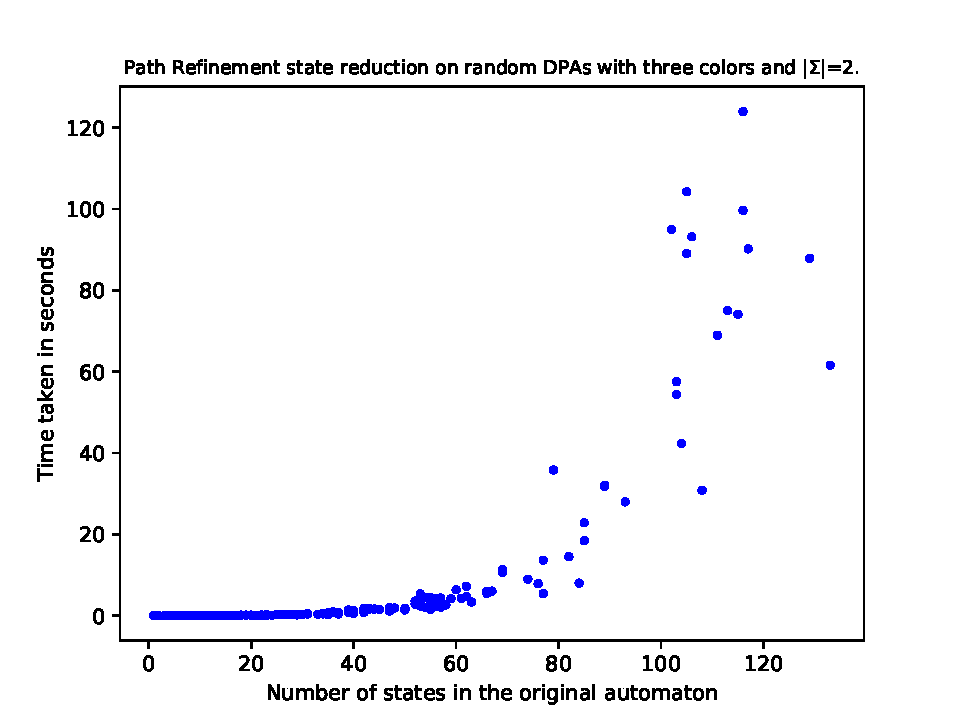
\includegraphics[page=1,height=.3\textheight]{../data/analysis/path_refinement/gendet_ap1.pdf} 
		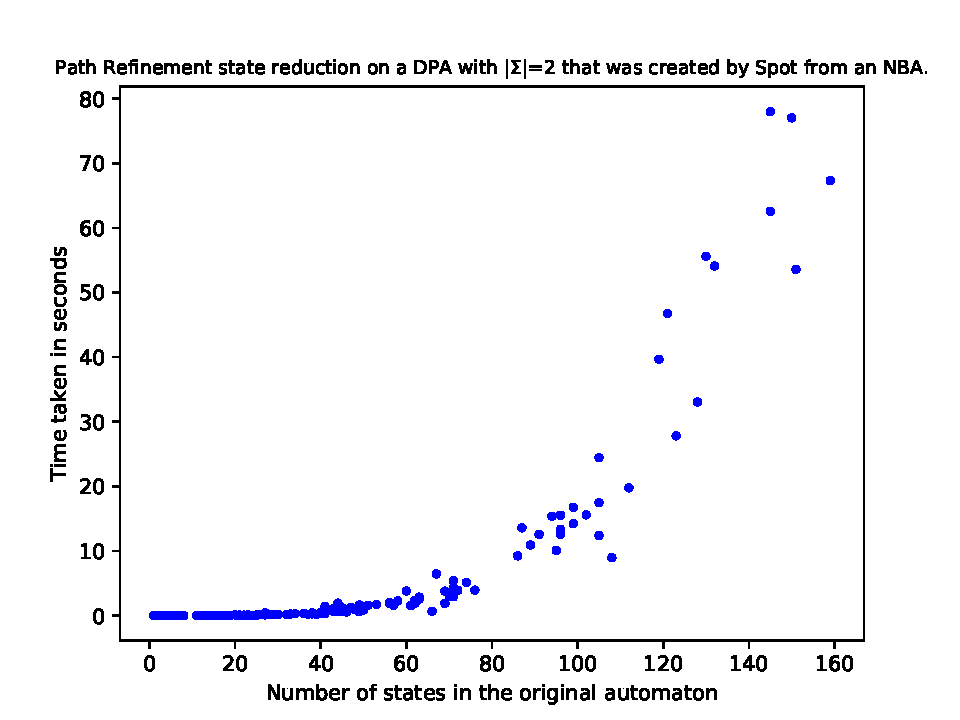
\includegraphics[page=1,height=.3\textheight]{../data/analysis/path_refinement/detspot_ap1.pdf} 
		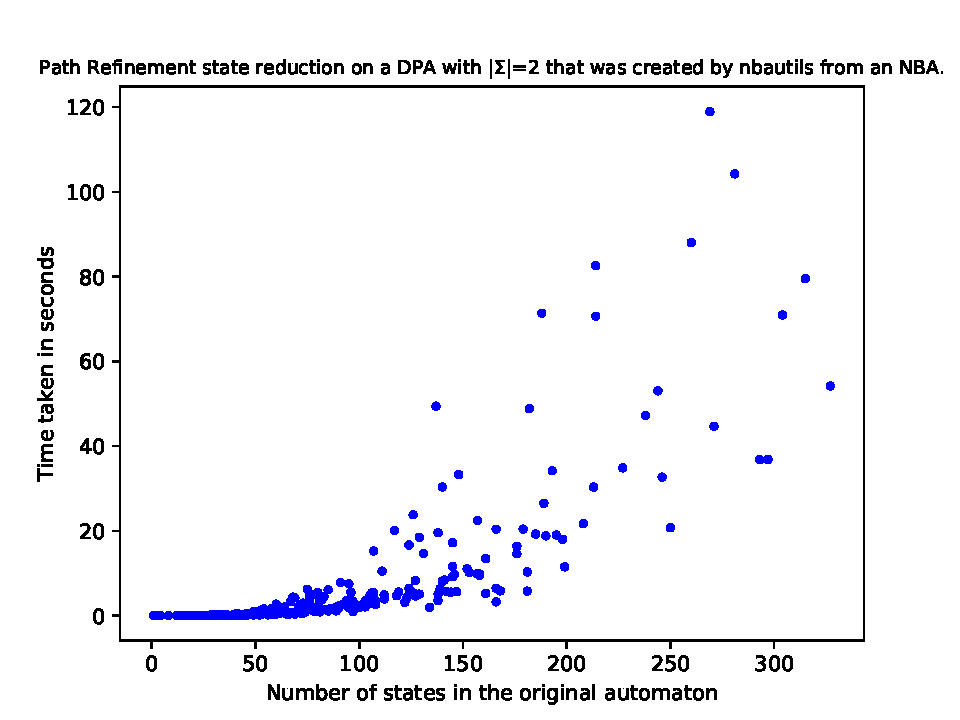
\includegraphics[page=1,height=.3\textheight]{../data/analysis/path_refinement/detnbaut_ap1.pdf} 
		\caption{Time of the state reduction of different automata using $\mu_\text{PR}^\lambda$.}
		\label{fig:pr:empirical_time}
	\end{minipage}
\end{figure}

\begin{figure}
	\centering
	\includegraphics[page=6,height=.4\textheight]{../data/analysis/path_refinement/detnbaut_safra_ap1.pdf} 
	\caption{State reduction of different automata using $\mu_\text{PR}^\lambda$.}
	\label{fig:pr:empirical_safra_size_hist}
\end{figure}

\begin{figure}
	\centering
	\includegraphics[page=3,height=.4\textheight]{../data/analysis/path_refinement/detnbaut_safra_ap1.pdf} 
	\caption{State reduction of different automata using $\mu_\text{PR}^\lambda$.}
	\label{fig:pr:empirical_safra_reduct_rel}
\end{figure}

\begin{figure}
	\centering
	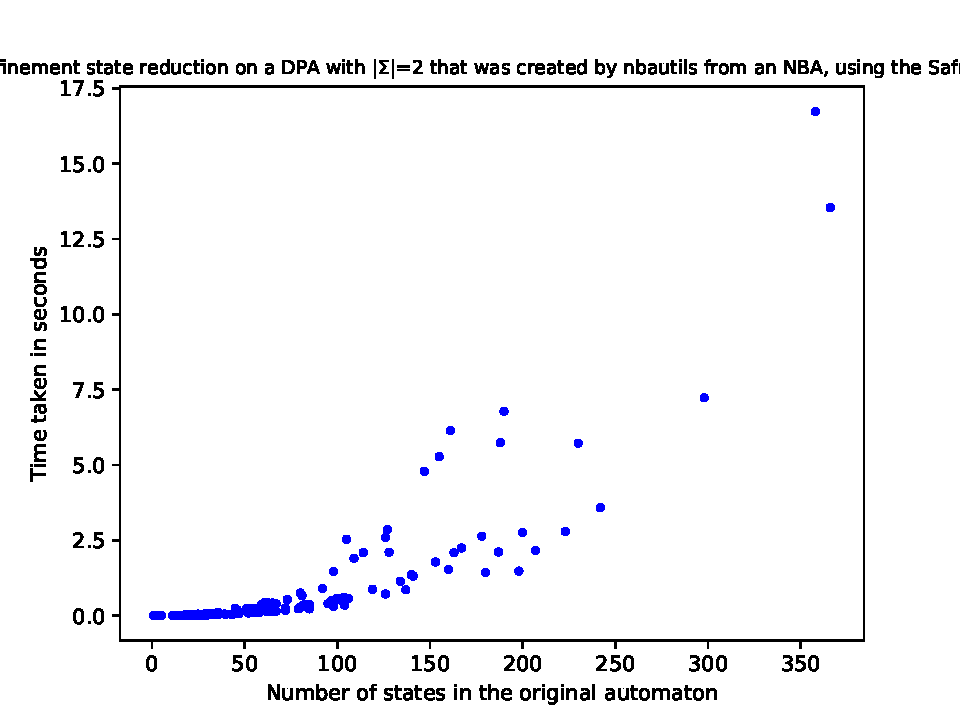
\includegraphics[page=1,height=.4\textheight]{../data/analysis/path_refinement/detnbaut_safra_ap1.pdf} 
	\caption{State reduction of different automata using $\mu_\text{PR}^\lambda$.}
	\label{fig:pr:empirical_safra_time}
\end{figure}




\section{Multiple Merges}
So far, we always considered $\mu_\text{PR}^\lambda$ for some fixed equivalence class $\lambda$. However, building this merger only touches states in $\lambda$; all other states of the automaton remain as before. 

From Theorem \ref{thm:pr:preserves_language}, we can deduce that if $R$ is a congruence relation that implies language equivalence on $\mathcal{A}$, then $R \cap (Q' \times Q')$ is the same on a representative merge $\mathcal{A}'$ (w.r.t. $\mu_\text{PR}^\lambda$). This tells us that we can simply \enquote{reuse} the relation $R$, or rather its equivalence classes, to compute the path refinement relation for different $\lambda$ and sequentially built their merges. The upcoming example shows that this can provide further state reduction and more importantly that the order that the equivalence classes are considered in matters.

The automaton displayed in figure \ref{fig:pr:example_lambda_order} has six states. Assume our relation has four classes, $\{q_1, q_5\}$, $\{q_2, q_3\}$, $\{q_4\}$, and $\{q_0\}$. Equivalence classes of size 1 cannot cause any state reduction, so we focus on $\lambda_1 = \{q_1, q_5\}$ and $\lambda_2 = \{q_2, q_3\}$.

Consider $\mathcal{A}_1$, a representative merge w.r.t. $\mu_\text{PR}^{\lambda_1}$. From $q_1$, there is a path back to $\lambda_1$ again that only visits priority 1, namely $q_1 q_3 q_4 q_5$. That is impossible from $q_5$, as the first step always leads to $q_0$ with priority 0. Hence, no merge will occur in this step.

On the other hand consider $\mathcal{A}_2$, a representative merge w.r.t. $\mu_\text{PR}^{\lambda_2}$. From the pair $(q_2, q_3)$, every path back to $\lambda_2$ will either move through $q_2$ or $q_0$ and thus have the minimal priority 0. The resulting automaton is shown in figure \ref{fig:pr:example_lambda_order2}.

Now look at $\mathcal{A}_{21}$, a representative merge of $\mathcal{A}_2$ w.r.t. $\mu_\text{PR}^{\lambda_1}$. As $q_3$ does not exist anymore, the path $q_1 q_3 q_4 q_5$ becomes $q_1 q_2 q_4 q_5$ with minimal priority of 0. In fact, now $q_1$ and $q_5$ can be merged, unlike before.

We were not able to find an easy heuristic to determine which order of classes gives the best reduction. One could of course repeat the reduction process over and over until no change is made anymore but that would bring the worst case runtime to about cubic in the number of states.


\begin{figure}
\centering
\begin{tikzpicture}[shorten >=1pt,node distance=2cm,on grid,initial text=]
  \node[state]           (0)                {$q_0,0$};
  \node[state]           (1) [right=of 0]   {$q_1,1$};
  \node[state]           (2) [below=of 0]   {$q_2,0$};
  \node[state]           (3) [right=of 2]   {$q_3,1$};
  \node[state]           (4) [right=of 3]   {$q_4,1$};
  \node[state]           (5) [above=of 0]   {$q_5,1$};
  \path[->] (0) edge node [above] {a} (3)
            (0) edge [bend left] node [above] {b} (1)
            (1) edge node [left] {a} (3)
            (1) edge [bend left] node [above] {b} (0)
            (2) edge [loop left] node {a} (2)
            (2) edge [bend right] node [below] {b} (4)
            (3) edge node [above] {a} (2)
            (3) edge node [above] {b} (4)
            (4) edge [bend right] node [above right] {a,b} (5)
            (5) edge node [left] {a,b} (0);
\end{tikzpicture}
\caption{Example automaton for which the order of congruence classes matters in path refinement.}
\label{fig:pr:example_lambda_order}
\end{figure}


\begin{figure}
\centering
\begin{tikzpicture}[shorten >=1pt,node distance=2cm,on grid,initial text=]
  \node[state]           (0)                {$q_0,0$};
  \node[state]           (1) [right=of 0]   {$q_1,1$};
  \node[state]           (2) [below=of 0]   {$q_2,0$};
  \node[state]           (4) [right=of 3]   {$q_4,1$};
  \node[state]           (5) [above=of 0]   {$q_5,1$};
  \path[->] (0) edge node [left] {a} (2)
            (0) edge [bend left] node [above] {b} (1)
            (1) edge node [left] {a} (2)
            (1) edge [bend left] node [above] {b} (0)
            (2) edge [loop left] node {a} (2)
            (2) edge node [below] {b} (4)
            (4) edge [bend right] node [above right] {a,b} (5)
            (5) edge node [left] {a,b} (0);
\end{tikzpicture}
\caption{Automaton from figure \ref{fig:pr:example_lambda_order} after merging $q_2$ and $q_3$.}
\label{fig:pr:example_lambda_order2}
\end{figure}















